\newpage
\section{Komplexe Funktionen}
\subsection{Exponential-/Logarithmusfunktion}\label{expfunc}
\[e^{j\alpha}= \cjs(\alpha) = \cos\alpha + j\sin\alpha\]

\[e^z= e^{z_1 + jz_2} = e^{z_1}\cdot e^{jz_2} = e^{z_1} \cdot \cjs(z_2) \qquad z \in \mathbb{C} \]
Realteil $z_1$ von $e^{z_1+jz_2}$ ist der Streckungsfaktor. Der Imaginärteil $z_2$ ist der zweite Term.

\subsection{Logarithmus und Potenzen}
\subsubsection{Logarithmus}\label{logfunc}
Der reelle Logarithmus hat den Wert $\ln(1) = 0$. Der komplexe Logarithmus ist definiert als:
\[\Ln(z) = \ln(\left|z\right|) + j\cdot arg(z) \]

\noindent\textbf{Achtung:} Im komplexen gibt es unendlich viele Lösungen für zB $\Ln(-j)= j(-\frac{\pi}{2} + 2k\pi)$. Auch in $\mathbb{C}$ ist $\Ln(0) = undef$ nicht definiert.

\subsubsection{Potenzen}\label{potfunc}
Potenzen mit komplexen Exponenten besitzen $\infty$-wertig Resultate, nur für $b \in \mathbb{Z}$ sind diese eindeutig.
\[
a^b = e^{b \cdot \Ln(a)} \qquad (a,b \in \mathbb{C};  a \neq 0)
\]
\textbf{Beispiel:} $z = (-j)^{2j} \Rightarrow e^{2j \cdot \Ln(-j)} = e^{\pi - 4k\pi}$

\subsection{Trigonometrie ($z \in \mathbb{C})$}
\[\sin(z) = \frac{e^{jz} -e^{-jz}}{2j} \quad \cos(a) = \frac{e^{jz} +e^{-jz}}{2} \quad \tan(z) = \frac{\sin(z)}{\cos(z)}\]

\subsection{Harmonische Schwingungen}
\[
z(t) = A \cdot e^{j(\omega t + \varphi)} = \underbrace{A \cdot e^{j\varphi}}_\text{Komplexe Amplitude} \cdot \underbrace{e^{j\omega t}}_{\text{Zeitfunktion}}
\]
\noindent Die Überlagerung von harmonischen Schwingungen können mittels Superpositions-Prinzip berechnet werden.

\noindent Beispiel:
\begin{align*}
	y_1 &= A\sin[\omega t + \varphi] &\qquad y_2 &= A\sin[\omega t + (\varphi + 120°)] \\
	&= A e ^{j(\omega t + j\varphi)} &\qquad  &= A e^{j(\omega t + \varphi - 120)}\\
	&= A e ^{j\omega t} \cdot \underbrace{e^{j\varphi}}_{K_1} &\qquad  &= A e^{j\omega t} \cdot \underbrace{e^{j(\varphi - 120)}}_{K_2}\\    
	\\
	y &= y_1 + y_2 &&= A e^{j\omega t} (K_1 + K_2) 
\end{align*}

\subsection{Abbildungen}
Um eine Abbildung $w$ durch eine Funktion $f$ auszudrücken, werden gegebene Komplexe Zahlen $z_i$ parametrisiert $r(z_i), c(z_i)$ und mit $f$ verrechnet.
\[z = r(z_i) + jc(z_i) \rightarrow f(z) = w \]

\subsubsection{Parametrisierung}
\subsubsection{Vektoren}
\begin{minipage}{\columnwidth}	
	\noindent\textbf{Geraden} parametrisierungen in der Gausschen-Zahlenebene können gleich wie Vektoren beschrieben werden. Wobei $r \in \mathbb{R}$ gilt.
		
	\begin{minipage}{0.6\textwidth}
		\begin{align*}
			\begin{pmatrix}z_1 \\ z_2\end{pmatrix} &= \begin{pmatrix}1 \\ 2\end{pmatrix} +  r \cdot \begin{pmatrix}1 \\ -1\end{pmatrix} \\
			z &= 1 + 2j + r \cdot (1-j) \\
		\end{align*}
	\end{minipage}%%% to prevent a space
	\begin{minipage}{0.4\textwidth}
		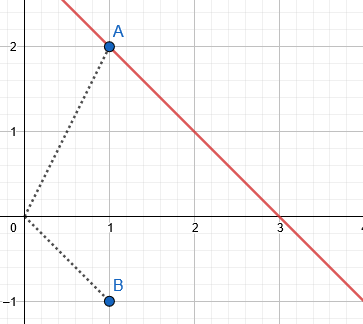
\includegraphics[width=\columnwidth]{Images/parameter_gerade}
	\end{minipage}
\end{minipage}
~\\
\begin{minipage}{\columnwidth}	
	\noindent\textbf{Kreise} können mithilfe der Eulerform dargestellt werden. Wobei $+t$ im gegen UZS und $-t$ mit UZS richtet:
	
	\begin{minipage}{0.6\textwidth}
		\begin{align*}
			z = m + r \cdot e ^{\pm jt} \qquad t \in [0; 2\pi)
		\end{align*}
	\end{minipage}%%% to prevent a space
	\begin{minipage}{0.4\textwidth}
		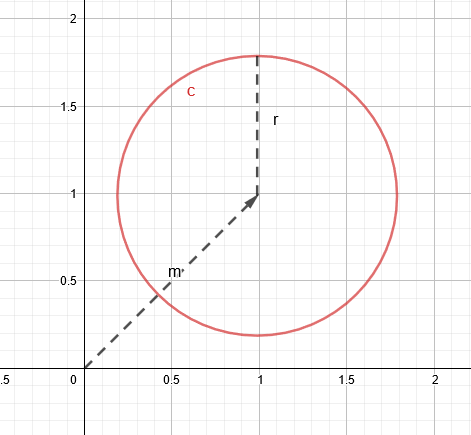
\includegraphics[width=\columnwidth]{Images/parameter_kreis}
	\end{minipage}
\end{minipage}

~\\
\begin{minipage}{\columnwidth}	
	\noindent\textbf{Ellipsen} können ähnlich wie Kreise mit Parameter $a,b \in \mathbb{R}$ parametrisiert werden:
	
	\begin{minipage}{0.6\textwidth}
		\begin{align*}
			z = a\cdot\cos(t) + j\cdot b \cdot \sin(t) \quad t \in [0; 2\pi)
		\end{align*}
	\end{minipage}%%% to prevent a space
	\begin{minipage}{0.4\textwidth}
		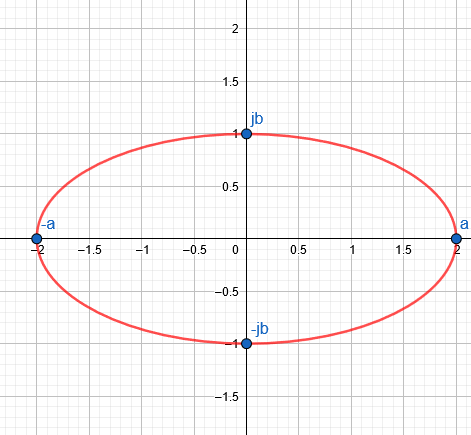
\includegraphics[width=\columnwidth]{Images/parameter_ellipse}
	\end{minipage}
\end{minipage}

\subsection{Ableitung}
Die Ableitung $f'$ in $\mathbb{C}$ entspricht einer Drehstreckung mit Faktor $f'$. Eine differenzierbare Funktion $f$ ist in allen Punkten mit $f'(z) \neq 0$ \textbf{winkeltreu}. Sie bewirkt dort eine Drehstreckung mit \textbf{Drehwinkel} $\arg(f'(z))$ und \textbf{Streckfaktor} $|f'(z)|$.

\subsection{Potenzfunktion $f(z) = z^n$}
In Polar-Koordinaten Darstellung werden die Winkel um das $n$-Fache verdoppelt, bzw. mit $\sqrt[n]{z}$ halbiert.
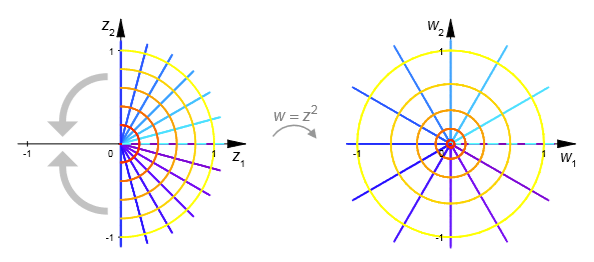
\includegraphics[width=\columnwidth]{Images/quadrat_funktion}

\subsection{Linearefunktion $f(z) = az + b$}
$b$ bewirkt eine Translation um den Ortsvektor $b$. $a$ bewirkt eine Drehstreckung mit Winkel $\arg(a)$ und Streckung mit $|a|$.
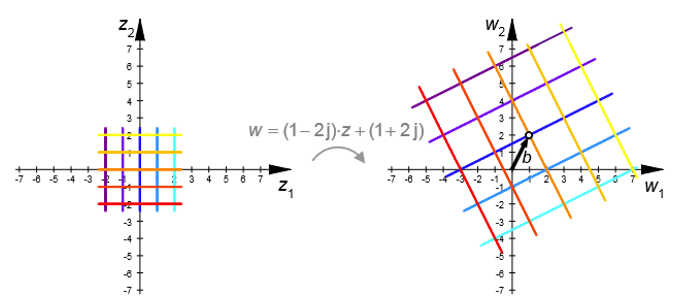
\includegraphics[width=\columnwidth]{Images/lineare_funktion}


\subsection{Kehrwertfunktion $f(z) = \frac{1}{z}$}
Bewirkt eine \underline{Kreisspiegelung} und mit der Definition $\frac{1}{\infty} = 0$ bzw. $\frac{1}{0} = \infty$ ist die Kehrwertfunktion überall in $\mathbb{C}\cup\{\infty\}$ winkeltreu. Viele Gebiete können via Rand mit folgenden Umformungen abgesteckt und bestimmt werden.

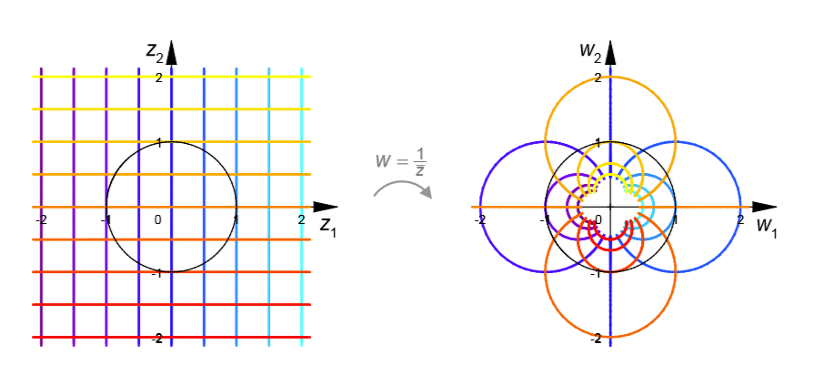
\includegraphics[width=\columnwidth]{Images/kehrwert_funktion}\\

Folgende möglichen Fälle sind zu unterscheiden:\\
\noindent (1) Gerade durch Ursprung $U$ beleibt gerade.\\
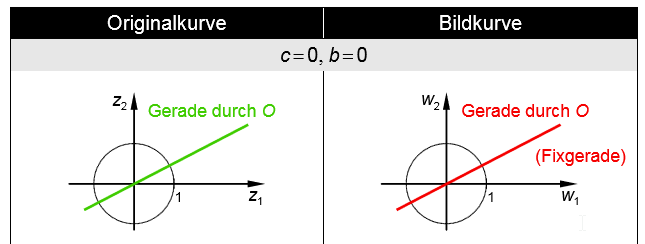
\includegraphics[width=\columnwidth]{Images/kreisspiegelung_gerade_o}

~\\
\noindent (2) Gerade $g$ nicht durch $U$ wird zu Kreis, Wobei Strecke des Schnittpunktes $S$ der orthogonale $g'$ mit $g$, $\frac{1}{s}$ gerechnet wird und diese den Radius von Kreis $k$ definiert.\\
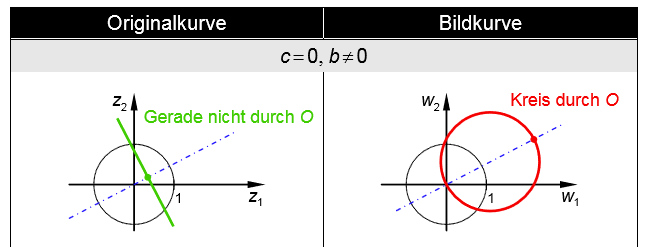
\includegraphics[width=\columnwidth]{Images/kreisspiegelung_gerade_no}

~\\
\noindent (3) Kreis durch $U$ wird zu Gerade. Dabei wird Strecke $s$ von Hilfsgerade $h$ und Schnittpunkt von Kreis $k$ $\frac{1}{s}$ gerechnet. Diese neue Strecke $s'$ definiert die orthogonale Gerade $g$\\
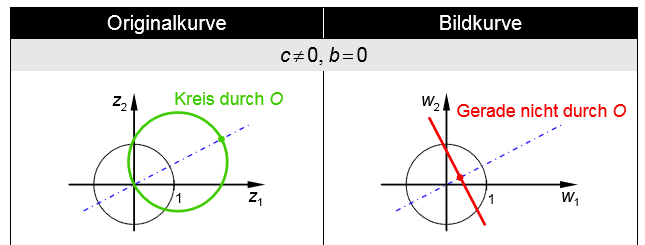
\includegraphics[width=\columnwidth]{Images/kreisspiegelung_kreis_o}

~\\
\noindent (4) Kreis nicht durch Ursprung bleibt Kreis. Der neue Kreis bleibt auf Hilfsgerade $h$ wobei Schnittpunkte und Mittelpunkt jeweils $\frac{1}{s}$ den neuen Punkt definieren. \\
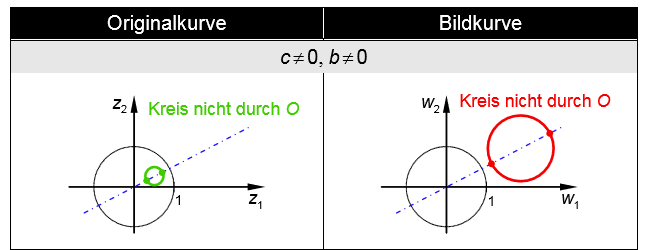
\includegraphics[width=\columnwidth]{Images/kreisspiegelung_kreis_no}

\subsection{Möbiustransformation $f(z) = \frac{az+b}{cz+d}$}
Die Möbius-Transformation ist eine Kombination aus:
\[
f: z \xmapsto[u=cz+d]{\text{Linear}} u \xmapsto[v=\frac{1}{u}]{\text{Kehrwert}} v \xmapsto[w=\frac{bc-ad}{c}v+\frac{a}{c}]{\text{Linear}}
\]

\includegraphics[width=\columnwidth]{Images/möbius_funktion}

\subsection{Joukowski-Funktion $f(z) = z + \frac{1}{z}$}
Bewegt weit weg vom Koordinatenursprung unwesentlich, hingegen nahe Punkte werden zusammen gedrückt.\\
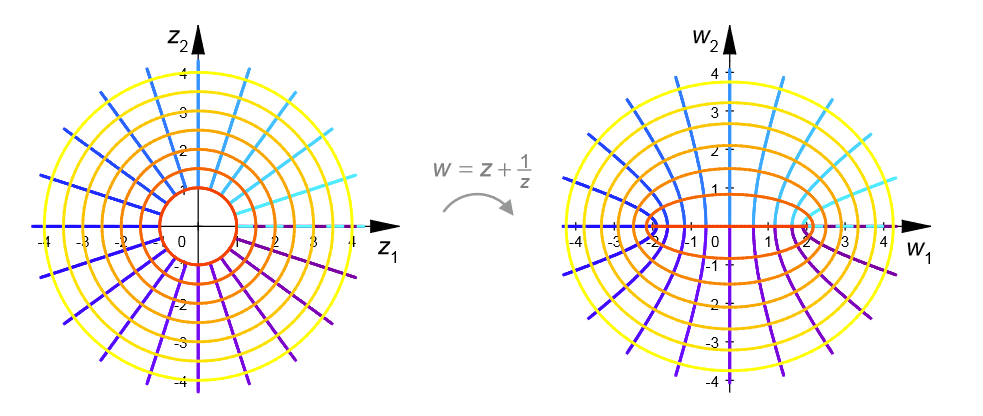
\includegraphics[width=\columnwidth]{Images/joukowski_funktion}

\subsection{Exponentialfunktion-Funktion $f(z) = e^z$}
Die Exp-Funktion ist $2\pi j$-Periodisch. Die Waagrechten Gitternetzlinien bilden Strahlen vom Koordinatenursprung weg, senkrechte Gitternetzlinien hingegen gehen zu konzentrischen Kreise um den Ursprung über.\\
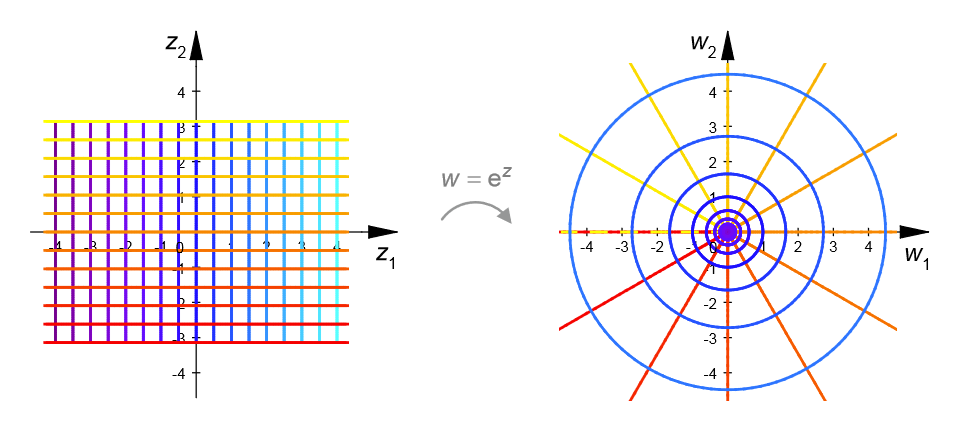
\includegraphics[width=\columnwidth]{Images/exp_funktion}


\subsection{Trigo-Funktion $f(z) = sin(z)$}
Da bereits $e^z$ $2\pi j$-Periodisch ist, sind auch die Trigonometrischen Funktionen periodisch. Die Gitternetzlinien gehen zu Ellipsen und Hyperbeln über.
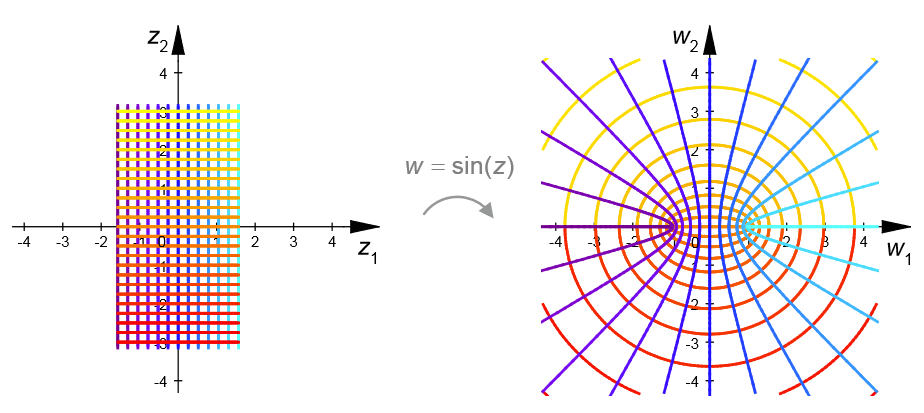
\includegraphics[width=\columnwidth]{Images/sinus_funktion}